
\section{Exercises}
\label{app:A-exercises}

\begin{exercise}\label{ex:1chap1}
Let $P=[p,q,r] $ be an interior point of an equilateral triangle $T=ABC$.

\noindent i) Show that the distances of $P$ to the sidelines of the triangle $T$ are given by
\[ [pk,qk,rk], \;\;\;k=\frac{2\Delta}{pa+qb+rc}\]
where $\Delta$ is the area of the triangle.

 \noindent ii)
 Show that  $k(p+q+r)$ is equal to the length of the triangle's altitude, i.e., the sum is independent of the position of the point.
 
 \noindent iii) Show that the same result is true when $P$ is an exterior point, but here we need to consider distances with signal, according to the position of $P$. See \cref{fig:trilinear_signal}.
 
 \noindent iv) Show that the reciprocal is true, i.e., if the sum of distances is independent of the point, then the triangle is equilateral.
 
 \noindent iv) Generalize items ii), iii) and iv)  for regular polygons.
 \end{exercise}
 
 \begin{exercise}\label{ex:2chap1} Show that $X_i$??  of the reference triangle    is the symmedian point of its excentral triangle.
 
  \end{exercise}
 
  \begin{exercise}\label{ex:3appA}
 Let $ABC$ be a  triangle and    $P$ and $Q$ be isogonal conjugates.  Then the circumcenters of the triangles $BPC$ and $BQC$ are inverses with respect to the circumcircle of the triangle $ABC$.
   \end{exercise}
  
   \begin{exercise}\label{ex:4appA}
   Let $P$ and $Q$ be isogonal conjugates in the interior of
the triangle $ABC$. Then the   pedal  triangles of $P$ and $Q$
 share a circumcircle. Moreover, the center of this circle is the midpoint
of $PQ$.
    \end{exercise}
   
      \begin{exercise}\label{ex:5app}
  Let $P $ and $Q$ isogonal conjugates.  If the point
is reflected about the sides
$AB$, $BC$ and $AC$.
  Then the resulting triangle has circumcenter the point $P$.
 
    \end{exercise}  \begin{exercise}\label{ex:6app}
  Let $\mathcal{E}$ be an ellipse inscribed in a triangle $ABC$. Then foci $F_1$ and $F_2$ of $\mathcal{E}$ are isogonal conjugates. 
 
    \end{exercise}
    
     \begin{exercise}\label{ex:7app}
 Consider two lines $x$ and $y$ passing through $P_0$.
 Let $ u$ and $v$ conjugate lines with respect to $x$ and $y$. Let $P\in u$ and $P_x\in x$ and $P_y\in y$ the pedal points of $P$. 
 
 \noindent i) Show that the points $\{P_0,P,P_x,P_y\} $
 are con-cyclic.
 
 \noindent ii) Show that the line $h=P_xP_y$ is orthogonal to the line $v$. See \cref{fig:isogonal_orthogonal}. 
 
 \begin{figure}[H]
    \centering
   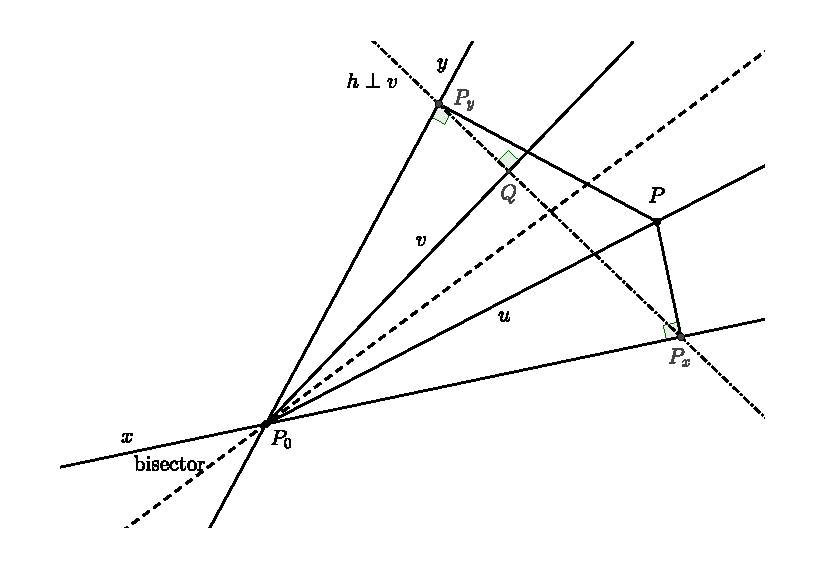
\includegraphics[scale=0.7]{pics_appA_0910_isogonal_ortogonal_conjugateline.pdf}
    \caption{ Isogonal line $v$ is orthogonal to  $h=P_xP_y$.
    \label{fig:isogonal_orthogonal}
    }
\end{figure}
 
    \end{exercise}
    
         \begin{exercise}\label{ex:8app}
         Show that the Brocard points can be  constructed as shown in \cref{fig:brocard_construction}.
         
         Consider a triangle $ABC$ and draw a line passing through $A$ and parallel to $BC$. Consider also a circle passing through $C$ and tangent to the line $AB$ at the vertex $A$. The point $D$ is the intersection of the line and circle constructed above.  The line $BD$ intersect the circle at the Brocard point $\Omega_1$ of $ABC$. Repeat this construction for the other vertices and obtain $\Omega_2.$
     
 \begin{figure}[H]
    \centering
   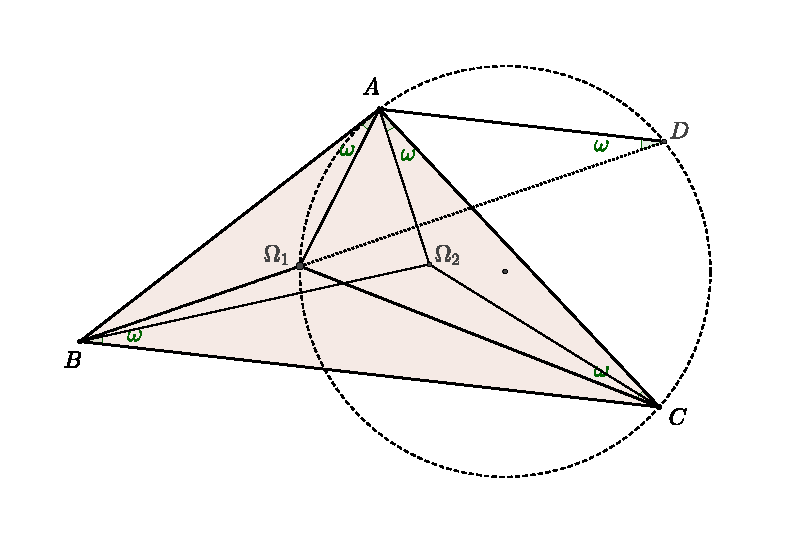
\includegraphics[scale=0.7]{zappA/pics/pics_appA_0930_brocard_points_construcao.pdf}
    \caption{ Geometric construction of Brocard points
    \label{fig:brocard_construction}
    }
\end{figure}
 
    \end{exercise}
    
    \begin{exercise}
      Let the incircle of triangle $ABC$ touch side $ BC$ at $A_1$, and let $A_1 A_1'$ be a diameter of the incircle.
Denote by $A_2$ the intersection of the lines $AA_1'$  and d$BC$. Show that   $BA_2  = CA_1$.

Consider the similar construction with respect to the two other sides.
Show that the three lines $AA_2$, $BB_2$ and $CC_2$ are concurrent. Show that this point is  $X_8$ and that it belongs to the line $X_1X_6$. 


 \end{exercise}
 
 \begin{exercise}
 A    similarity    about a point $O$   is a composition of a
rotation and a dilation, both centered at $O$.
Consider a quadrilateral   $ABCD$  which is not a parallelogram.  

Show that there is a unique   similarity sending $AC$ to $BD$. 

Let $A, B, C, D$  be four distinct point in the plane, such that $AC$ is not parallel to $BD$. Let $X$ be the the intersection of
  $ AC$ and $BD$.  Let the circumcircles of $ABX $ and $CDX$ meet again at $O$. Then $O$  is the
center of the unique   similarity that sends $A $ to $C$ and $B $ to $D$.

If $O$ is the center of the   similarity that sends $A$ to $C$ and $B$ to $D$, then $O$ is also the center
of the   similarity that sends $A$ to $B$ and $C$ to $  D$.
See \cite{zhao-2021} and \cite{caliz2020-area-product}.
%\noindent Hint: use complex numbers.
%See https://yufeizhao.com/olympiad/three\_%geometry\_lemmas.pdf
\end{exercise}

\begin{exercise}
Let $ABC$ be a triangle and $\mathcal{C}$  its circumcircle. Let the tangent lines to $\mathcal{C}$  at $B$ and $C$ meet at $D$.
Show that   $AD $ is  a symmedian of $ABC$.
 Use this fact to construct $X_6$.
\end{exercise}

\begin{exercise}
Consider a triangle $ABC$ and in the sideline $BC$, construct two points $A_1$, $A_2$ such that $A_2-C=c$ and $A_1-B=b$. The segment $A_1A_2$ has length $a+b+c$. Repeat the construction for the other two sidelines. Show that the six points obtained lies in a circle, known as Conway's circle.
\end{exercise}

\begin{exercise}
A polar circle of an obtuse triangle $T=ABC$ is the  circle centered at $H=X_4$ (orthocenter) and radius $r$ given by
\[ r^2=4R^2-\frac{1}{2}(a^2+b^2+c^2)\]
where $R$ is the radius of the circumcircle of $T$. Define analogously the polar circles of the triangles $ABH$, $BCH$ and $ACH$. Show that all polar circles intersect orthogonally, see \cref{fig:pics-appA-polarcircles}.
Determine the nine-point-circles of the four triangles.

\begin{figure}
    \centering
    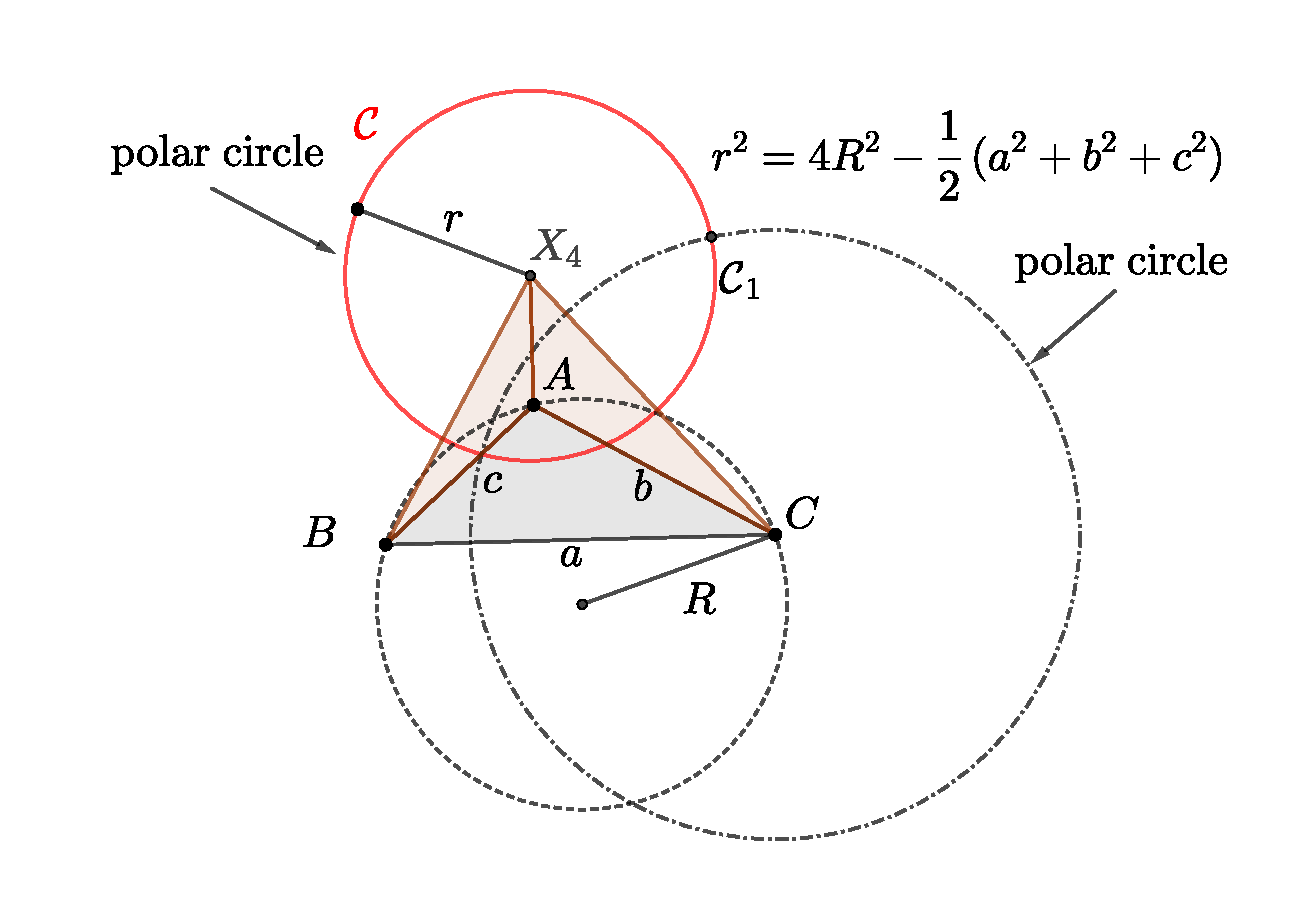
\includegraphics[scale=0.4]{zappA/pics/pics-appA-108-polar-circle-ortocentro.pdf}
    \caption{Polar circles intersecting orthogonally.}
    \label{fig:pics-appA-polarcircles}
\end{figure}

An orthocentric system is a set of four points $P_i=(x_i,y_i)$ $ (i=1,\ldots,4)$ in the plane such each point $P_i$ is the orthocenter of the triangle defined by the other three points. Show that the set of orthocentric systems is an algebraic set  of codimension 2 in $\mathbb{R}^8$.
\end{exercise}

\begin{exercise}
Show that the circumconic that is the isogonal image of Euler line is never an ellipse. 
\label{ex:appA-isogonal-euler}
\end{exercise}

\begin{exercise}
Consider the triangle $A=[\alpha,\beta]$, $B=[-1,0]$
and $C=[1,0]$ in cartesian coordinates with sides
$a=2,\, b=\sqrt{(\alpha-1)^2+\beta^2}, \, c=\sqrt{(\alpha+1)^2+\beta^2}$.

Let   $P_1=[p_1,q_1,r_1]$ and $P_2=[p_2,q_2,r_2]$ defined in trilinear coordinates.
 
Let $P(u)=u P_1+(1-u) P_2 $ and consider the conversion of these points in cartesian coordinates given by \cref{eqn:appAtrilin-cartesian}.
Let $X(P_1)=P_1^*$ and $X(P_2)=P_2^*$
Show that $P^{*}(u)=X(P(u))$ is a straight line which has the same locus of $w P_1^{*}+(1-w)P_2^{*}$. Find the relation between the parameters $u$ and $w$, obtaining that $w=k_1 u/((k_1 -k_2)u+k_2)$.
\end{exercise}

\begin{exercise} Show that the
 antiorthic axis of a triangle $ABC$ is orthogonal to the line $X_1X_3$.
\end{exercise}

\begin{exercise} Consider a triangle center given in  barycentric coordinates as $P=[f(a,b,c),f(b,c,a), f(c,a,b)]$ and define the point $E(P)=[f(-a,b,c),f(b,c,-a), f(c, -a,b)]$. 
Show that $E $ is an involution   and   that $X_2$ is a fixed point of $E$. 

Determine the points $E(X_1)$, $E(X_3)$ and $E(X_4)$. See \cite{etc}.
 
 
\end{exercise}